\providecommand{\HeadlineResult}{The locked real-study matrix and its fail-closed audits are still in progress; no empirical headline is claimed in this source state.}
\providecommand{\PointViolationRate}{pending}
\providecommand{\VERAViolationRate}{pending}
\providecommand{\SafeRetentionRate}{pending}
\providecommand{\OfficialReceiptCount}{pending}
\providecommand{\SeedBlockedResult}{pending}
\providecommand{\CodeAvailabilityText}{Code, hashed preregistrations, compact receipts, audit scripts, and manuscript sources are included in the anonymous supplementary archive. Large public-dataset derivatives are represented by manifests and content hashes.}

\begin{abstract}
Concept erasers can suppress sensitive information in a representation while
damaging its target task or failing under deployment shift. The eraser alone
does not answer the deployment question: under what shift, if any, is an edit
still supported by evidence? We introduce VERA, Verified Erasure under
Reweighting Ambiguity, a decision layer that audits target loss on paired
identity/edit outcomes and sensitive leakage with fresh heterogeneous
attackers. For each registered edit, VERA reports a simultaneous support-aware
envelope of environment and source-conditional density-ratio budgets under
which all target-harm and balanced-leakage contracts hold, together with a
more powerful fixed-profile decision, or returns \textsc{Abstain}. We prove
uniform envelope validity, permit arbitrary mixtures of observed environments
and arbitrary source-prior shift, and show that no validation-only protocol can
nontrivially certify unconstrained deployment mass outside its support.
Finite-family testing and abstention are inherited from Learn Then Test style
risk control, not claimed as new. The empirical protocol combines a 54-cell
exact abstention study, a 216-cell candidate-family/group-count coverage grid,
and a preregistered 200-run official-code matrix spanning five erasers, five
datasets, and eight untouched seeds. \HeadlineResult
\end{abstract}

\section{Introduction}

Representation editing is an intervention. It changes what downstream models
can recover from a frozen representation, often to remove a protected,
nuisance, or source concept. INLP, R-LACE, LEACE, kernel methods, TaCo, SPLINCE,
and MANCE++ provide increasingly expressive ways to construct such edits
\cite{ravfogel2020null,ravfogel2022linear,belrose2023leace,ravfogel2022kernel,jourdan2023taco,holstege2025splince,avitan2026mance}.
Their successes do not make every resulting edit deployable. Removing a
correlated concept can damage the target, a probe used by the eraser can
understate leakage to a different attacker, and an IID validation result need
not survive reweighting at deployment.

This paper asks a narrower, operational question: what is the largest declared
shift under which one candidate edit can be certified to preserve the target
while limiting all registered leakage attackers? The target audit is paired.
For the same example, it subtracts the identity representation's zero-one loss
from the edited representation's loss, isolating incremental harm rather than
conflating it with baseline error. The shift class is stratified: within each
environment, the target law has a bounded density ratio relative to its
certification law. Leakage is the equal mean of two robust source-class
recalls, each under a bounded source-conditional density ratio. Environment
weights and source prevalence may therefore vary arbitrarily; ordinary
prevalence-weighted accuracy is not the contract. At a declared profile, VERA
uses a candidate-wise intersection--union test. Separately, it simultaneously
upper-bounds every candidate-contract curve and inverts them into a
support-aware shift envelope and common radius $\widehat\Gamma_e$. A zero
radius means that even the IID contract is not established. New support forces
abstention.

The statistical mechanism must be positioned carefully. Risk-controlling
prediction sets, Learn Then Test (LTT), Conformal Risk Control, and Pareto
Testing already calibrate finite algorithm families against one or several
risks; recent work also couples risk, acceptance, and utility and provides
group-conditional PAC control
\cite{bates2021rcps,angelopoulos2025ltt,angelopoulos2024crc,laufer2023pareto,yu2026joint,huang2026conditional}.
Weighted risk control and robust validation already address important forms of
covariate and distribution shift
\cite{tibshirani2019covariate,almeida2025hprc,cauchois2024robust,ai2024finegrained}.
VERA uses these foundations. Its proposed contribution is the
representation-intervention object they do not report: a simultaneous,
support-aware envelope of groupwise reweighting budgets for paired edit harm
and an entire retrained-attacker portfolio. The common shift radius is one
summary of that envelope; unsupported required cells mark the boundary at which
it cannot be identified.

Our contributions are threefold. We robustify balanced accuracy into a
source-prior-invariant leakage contract and certify its joint support-aware envelope with
environment-conditional paired harm over a continuum of deployment budgets.
We formalize unsupported-environment abstention by an indistinguishability
theorem rather than a heuristic. We then test whether certification changes
deployment decisions in a locked cross-modal study with official INLP,
R-LACE, LEACE, TaCo, and MANCE++ code. All numbers are regenerated from
per-run receipts; internal audits are not substitutes for scientific review.

\begin{figure*}[t]
\centering
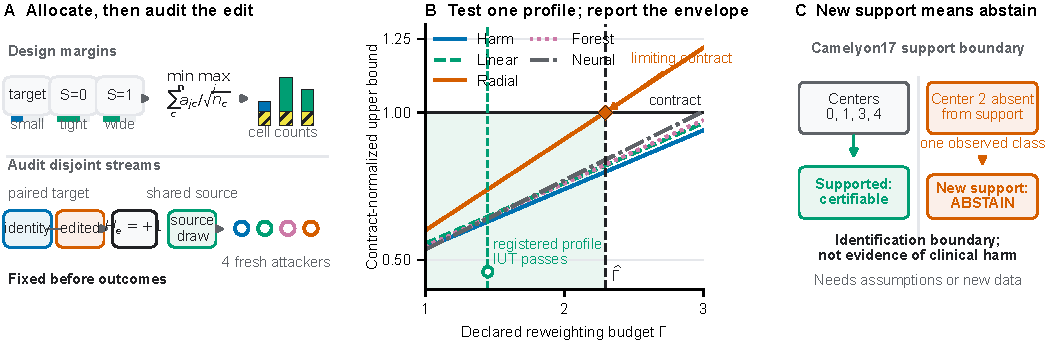
\includegraphics[width=\textwidth]{../../figures/vera_method_overview.pdf}
\caption{\textbf{VERA certifies an edit only within a declared, supported shift
class.} (A) Target harm compares identity and edited predictions on the same
examples; fresh heterogeneous attackers measure equal-weight source-class
recall. (B) At a fixed profile, every component must pass the candidate IUT;
simultaneous upper-risk curves are separately inverted to obtain the shift
envelope and limiting common radius. Curves are schematic. (C) The guarantee cannot cross new
support. In the registered Camelyon17 split, certification observes centers 0,
1, 3, and 4, while external center 2 is absent, so a five-center deployment
claim requires abstention unless an additional cross-center assumption is
supplied.}
\label{fig:overview}
\end{figure*}

\section{Related Work}

\paragraph{Concept erasure and probing.}
Linear erasure includes iterative nullspace projection, adversarial
low-rank projection, and the closed-form LEACE solution
\cite{ravfogel2020null,ravfogel2022linear,belrose2023leace}. Kernel erasure,
rate-distortion objectives, unaligned-attribute removal, TaCo, SPLINCE, and
MANCE extend the construction space
\cite{ravfogel2022kernel,chowdhury2023kram,shao2023unaligned,jourdan2023taco,holstege2025splince,avitan2026mance}.
Nonlinear guardedness can remain after linear removal, while perfect erasure
faces fundamental utility limits
\cite{akbari2025obliviator,chowdhury2025limits}. FARE and MMD-B-Fair provide
important certificates for restricted fair-representation objectives
\cite{jovanovic2023fare,deka2023mmdbfair}. VERA neither replaces these erasers
nor certifies absence of all information. It audits their candidate outputs
against a fixed portfolio. That portfolio follows the broader lesson that a
probe's result depends on its hypothesis class and training protocol
\cite{hewitt2019control,pimentel2020probing,voita2020mdl,elazar2021amnesic}.

\paragraph{Risk control and abstention.}
LTT turns calibration into testing over a finite family, and Pareto Testing
extends the view to multiple risks and objectives
\cite{angelopoulos2025ltt,laufer2023pareto}. Conformal Risk Control treats
general monotone losses \cite{angelopoulos2024crc}. Joint adaptive certificates
couple risk, acceptance, and utility, while group-conditional PAC methods
control routing risk within registered groups
\cite{yu2026joint,huang2026conditional}. These works invalidate any claim that
VERA invents finite-family, joint, or groupwise acceptance. Selective
classification and SelectiveNet reject individual examples
\cite{elyaniv2010foundations,geifman2017selective,geifman2019selectivenet}; VERA
instead rejects an entire intervention. Continuous monitoring detects risk
violations after deployment \cite{timans2025monitoring}, whereas VERA is a
predeployment, support-scoped sensitivity certificate.

\paragraph{Distribution shift and robust evaluation.}
Known importance weights can restore conformal or high-probability risk control
under a specified covariate shift
\cite{tibshirani2019covariate,almeida2025hprc}. Robust validation and
fine-grained robust conformal inference provide ambiguity-set guarantees
\cite{cauchois2024robust,ai2024finegrained}, while robust model evaluation and
CVaR concentration supply closely related technical tools
\cite{najafi2025federated,thomas2019cvar,waudbysmith2024means}. Distributional
fairness certificates and Wasserstein fairness audits are close application-level
neighbors \cite{kang2022certifying,ehyaei2025fragile}; concept interventions can
also fail under OOD leakage \cite{zarlenga2025leakage}. Worst-case subpopulation
treatment effects are especially close to our paired-harm view
\cite{jeong2020worstcase}. VERA does not claim these tools or generic robust
fairness auditing. It applies bounded reweighting to a selected representation
edit's paired target and retrained-attacker contracts and reports the admissible
support-scoped envelope. Group DRO and robustness benchmarks motivate the observed-group view
\cite{sagawa2020groupdro,koh2021wilds,zhou2021spurious,sohoni2020subclass}, and
domain-adaptation impossibility results motivate explicit support assumptions
\cite{bendavid2010impossibility,subbaswamy2021evaluation}.

\section{Problem Setup}

Let $Z\in\mathbb{R}^d$ be a frozen representation, $Y$ its target label, and
$S$ a source or sensitive label. An edit $e\in\mathcal E$ is fitted without the
certification fold and maps $Z$ to $Z^e$. The identity is $e=0$. Fresh target
models are fitted after every edit. For certification example $i$, define
paired target harm
\begin{equation}
H_{e,i}=\mathbf 1\{f_e(Z_i^e)\ne Y_i\}-
\mathbf 1\{f_0(Z_i)\ne Y_i\}\in\{-1,0,1\}.
\end{equation}
In the real protocol, identity is the paired comparator rather than a selectable
erasure action. If a deployment protocol may select identity, it must register
identity as one additional candidate in the finite-family correction; the
separate family-size coverage grid does so.
For each preregistered attacker $a\in\mathcal A$, let
$L_{e,a,i}=\mathbf 1\{a_e(Z_i^e)=S_i\}\in\{0,1\}$. Attackers are retrained
after each edit using construction data, but are fixed before certification
outcomes are used.

For validation law $P$ and $\Gamma\ge1$, define
\begin{equation}
\begin{aligned}
\mathcal Q_\Gamma(P)&=\left\{Q\ll P:0\le
\frac{\mathrm dQ}{\mathrm dP}\le\Gamma\quad P\text{-a.s.}\right\},\\
\rho_{\Gamma,P}(V)&=\sup_{Q\in\mathcal Q_\Gamma(P)}\mathbb E_Q[V].
\end{aligned}
\end{equation}
The target contract uses $P_g$, the certification law conditional on
environment $g$. For binary source, leakage uses the balanced robust accuracy
\begin{equation}
B_{e,a}(\eta_0,\eta_1)=\frac12\sum_{s\in\{0,1\}}
\rho_{\eta_s,P_s}(L_{e,a}),
\end{equation}
where $P_s$ is source-conditional. Balanced accuracy itself is standard
\cite{brodersen2010balanced}; our change is to robustify each recall and couple
the resulting attacker contracts to paired edit harm. A constant attacker
scores $1/2$, not one, and changing source prevalence does not change the
estimand. At zero or unit prevalence this is a standardized two-conditional
functional, not ordinary accuracy observable in an absent class. The population
common erasure shift radius is
\begin{equation}
\begin{aligned}
\Gamma_e^\star=\sup\{\Gamma\ge1:
&\rho_{\Gamma,P_k}(V_{e,k})\le c_k\\
&\text{for every registered contract }k\},
\end{aligned}
\end{equation}
with value zero if a contract fails at $\Gamma=1$.

\section{VERA}

The bounded-reweighting risk has the CVaR dual
\begin{equation}
\rho_{\Gamma,P}(V)=\inf_{\eta\in[a,b]}
\left\{\eta+\Gamma\mathbb E_P[(V-\eta)_+]\right\}.
\end{equation}
For general bounded variables, a Dvoretzky--Kiefer--Wolfowitz band gives a
uniform upper curve. Our discrete audit variables admit tighter exact curves.
For Bernoulli leakage with success probability $p$,
$\rho_{\Gamma,P}(L)=\min(1,\Gamma p)$. For paired harm with probabilities
$(p_-,p_0,p_+)$ on $(-1,0,1)$, set $a=\Gamma p_+$ and
$b=\Gamma(1-p_-)$. The adversary places its permitted mass on $+1$, then
zero, then $-1$:
\begin{equation}
\rho_{\Gamma,P}(H)=
\begin{cases}
1,&a\ge1,\\
a,&a<1\le b,\\
a+b-1,&b<1.
\end{cases}
\end{equation}
VERA substitutes one-sided Clopper--Pearson bounds. For paired harm it uses an upper bound
$U_+$ for $p_+$ and lower bound $L_-$ for $p_-$, clips
$\widetilde p_+=\min(U_+,1-L_-)$ to preserve the simplex, and splits the
component error between the two tails. Balanced leakage averages two class
recall bounds, splitting its component error between the source classes.

At the fixed deployment profile, each candidate is an intersection--union
test: all of its target and balanced-leakage components must pass at level
$\delta/|\mathcal E|$. If a candidate is unsafe, false acceptance implies
undercoverage of at least one fixed violated component. A union bound is needed
over candidates, but not over components. The separately reported envelope
uses Bonferroni coverage over every candidate--contract pair because every
curve remains available for post-certification inspection.

\begin{algorithm}[t]
\caption{VERA fixed-profile selection and shift envelope}
\label{alg:vera}
\begin{algorithmic}[1]
\REQUIRE Registered edits $\mathcal E$, contracts $c_k$, error $\delta$,
budget cap $\Gamma_{\max}$
\STATE Fit every edit, target model, and leakage attacker without certification outcomes
\STATE Allocate $\delta/|\mathcal E|$ to each candidate's fixed-profile IUT
\FOR{each edit $e$}
\STATE Accept the profile only if every component bound clears its threshold
\STATE Separately construct simultaneous curves and envelope $\widehat{\mathcal E}_e$
\ENDFOR
\RETURN the registered utility-best accepted edit, its envelope, or \textsc{Abstain}
\end{algorithmic}
\end{algorithm}

\begin{theorem}[Fixed-profile VERA]
Fix $M$ candidate edits and all audit variables independently of certification.
At one declared shift profile, accept a candidate only if every component
upper bound clears its threshold at level $\delta/M$. Then the probability of
deploying any candidate that violates at least one declared target or balanced
leakage contract is at most $\delta$.
\end{theorem}

For an unsafe candidate, fix one violated population component. Accepting that
candidate implies undercoverage of this component; intersecting more tests
cannot increase that probability. Union bounding only over the $M$ candidates
proves the result. This is the LTT-style finite-family decision used for the
primary experiment.

The simultaneous envelope is richer but more conservative. It contains every
profile $(\boldsymbol\gamma,\boldsymbol\eta)$ for which each environment target
curve clears $\tau$ and each attacker's mean of two source-class curves clears
$\lambda$. Its coverage event is uniform over the continuum of profile
coordinates. Environment mixing preserves the target threshold by linearity,
and source prevalence does not enter balanced leakage. Restricting this
envelope to the diagonal gives the reported common radius. Full statements and
proofs are in the supplement.

\begin{theorem}[Unsupported-cell impossibility]
Suppose a required audit cell has zero validation probability, and the model
class contains safe and unsafe worlds that induce identical protocol
observations but disagree on the contract in that cell. If deployment may
concentrate there, any validation-only protocol with uniform false-acceptance
control $\delta$ accepts the edit in the safe world with probability at most
$\delta$.
\end{theorem}

The proof is a two-world indistinguishability argument. It applies to an unseen
environment or a missing environment--source-label cell; a single-class slice
cannot identify the omitted class's conditional leakage. Camelyon17 center 2
and its constant binary source label therefore trigger abstention. This does
not assert that the measured center-2 target outcome necessarily violates a
contract.

\section{Experimental Protocol}

An initial five-seed pilot exposed that maximum class recall gives a constant
attacker leakage one; those results are retained as an estimand audit and are
excluded from confirmation. The balanced study was then fixed in a committed,
hashed preregistration before any seed 5--12 run. It crosses five erasers
(INLP, R-LACE, LEACE, TaCo, MANCE++), five datasets (Waterbirds,
Camelyon17-WILDS, CivilComments-WILDS, Bios, GaitPDB), and eight untouched
seeds, totaling 200 official-method runs. The modalities span
natural images, medical images, text, and time series. Bios and CivilComments
audit known representation-bias settings
\cite{dearteaga2019bios,borkan2019civilcomments}; Camelyon17 is a reliability
benchmark, not clinical evidence. Each run records split hashes, train-only
preprocessing, its upstream commit and entry point, per-example audit-array
hashes, and the shared runner commit. Model cards, datasheets, auditing, and
reproducibility guidance motivate this receipt design
\cite{mitchell2019modelcards,gebru2021datasheets,raji2020auditing,pineau2021reproducibility}.

Each candidate retrains a logistic target probe and four leakage attackers:
logistic regression, an RBF Nystroem map followed by logistic regression, a
random forest, and a two-layer MLP. Certification uses fractions
$\{0.05,0.10,0.25,0.50,1.00\}$, target thresholds
$\tau\in\{0.05,0.10,0.20\}$, leakage thresholds
$\lambda\in\{0.60,0.70,0.80\}$ and $\delta=0.05$. The primary fixed profile
uses $\Gamma=1.0$ at the full certification size; a fixed $\Gamma=1.01$
sensitivity and the full simultaneous radius are also reported. We compare
always deploy, feasible point selection without intervals, VERA-IUT, the VERA
envelope, and an external oracle. External contract violation is reported
separately from procedural non-certifiability. Camelyon17 external balanced
leakage is \textsc{NA} because the slice has one source class, and VERA must
abstain because center 2 is absent during certification.

The exact balanced study contains 2,000 replicates in each of 54 cells: six
certification sizes, three $\delta$ levels, and three shift budgets. Its finite
multinomial/binomial law gives an analytic abstention probability before Monte
Carlo is observed. A separately hashed 216-cell grid varies certification size,
four eraser-family sizes plus identity, validated-environment count, and
$\delta$, with 2,000 repetitions per cell. The real learning-curve overlay is labeled as a
full-certification plug-in diagnostic, not independent theorem validation.
Threshold configurations share eight seed-level fits, so an exact one-sided
seed-blocked sign-flip test governs the point-selection comparison under its
paired sign-symmetry null, with Holm correction over the four externally
estimable datasets. A sign-only test is a lower-power sensitivity that does not
require magnitude symmetry.

\section{Results}

\IfFileExists{vera_main_results_narrative.tex}{
  \input{vera_main_results_narrative}
  \begin{table*}[t]
\centering
\small
\begin{tabular}{@{}lrrrr@{}}
\toprule
Rule & Deployments & Viol./deployed & Safe retention & Median radius \\
\midrule
Always deploy & 256/256 (100.0\%) & 126/256 (49.2\%) & 130/187 (69.5\%) & NA \\
Validation selection & 186/256 (72.7\%) & 19/186 (10.2\%) & 167/187 (89.3\%) & NA \\
IID LTT & 87/256 (34.0\%) & 0/87 (0.0\%) & 87/187 (46.5\%) & NA \\
Robust point estimate & 94/256 (36.7\%) & 1/94 (1.1\%) & 93/187 (49.7\%) & NA \\
Scalar robust certificate & 245/256 (95.7\%) & 125/245 (51.0\%) & 120/187 (64.2\%) & NA \\
VERA fixed profile & 48/256 (18.8\%) & 0/48 (0.0\%) & 48/187 (25.7\%) & 1.03 \\
VERA vector envelope & 38/256 (14.8\%) & 0/38 (0.0\%) & 38/187 (20.3\%) & 1.03 \\
VERA common radius & 6/256 (2.3\%) & 0/6 (0.0\%) & 6/187 (3.2\%) & 1.12 \\
External oracle & 187/256 (73.0\%) & 0/187 (0.0\%) & 187/187 (100.0\%) & NA \\
\bottomrule
\end{tabular}
\caption{Primary controlled-shift results at $\Gamma=1.1$, budget 4,000, and targeted allocation with a 15\% evidence floor. Safe retention is retained oracle-safe opportunities over all oracle-safe opportunities. The primary result is mixed: VERA has zero deployed violations, but the preregistered usefulness lower bound is below the 20\% gate.}
\label{tab:controlled-main}
\end{table*}

  \begin{figure*}[t]
  \centering
  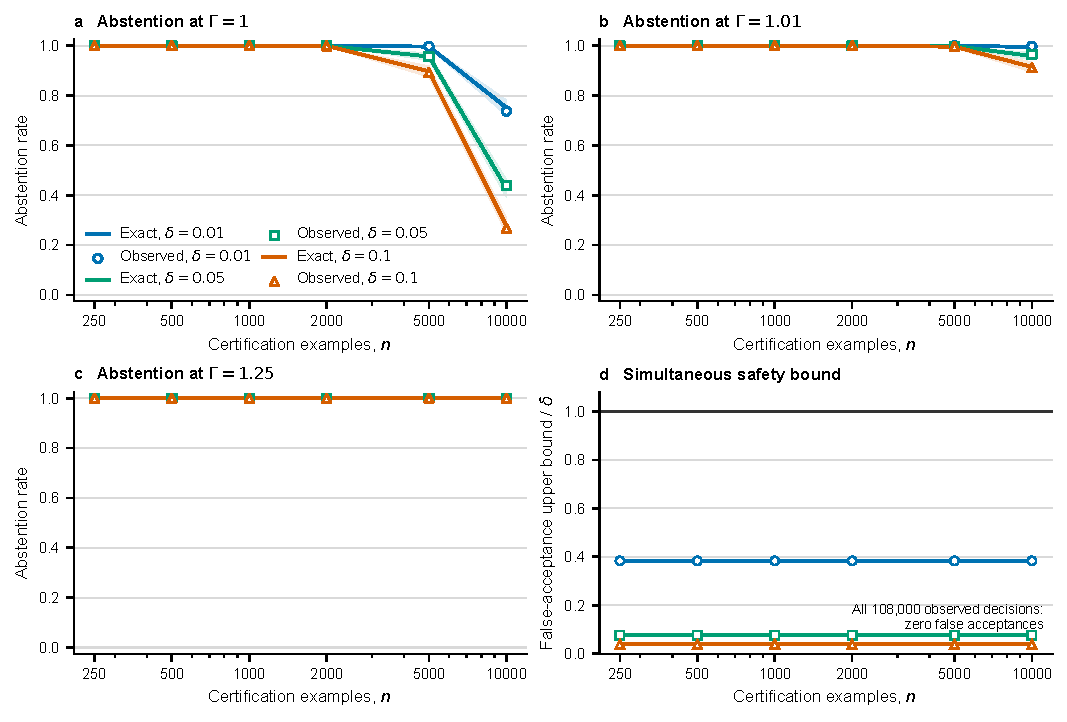
\includegraphics[width=\textwidth]{../../figures/vera_exact_theory_match.pdf}
  \caption{\textbf{Exact theory--data match.} Observed abstention from 2,000
  repetitions in each of 54 cells overlays the exact prediction; bands are simultaneous
  over all registered certification sizes. The independent replay verifies
  every random draw and false-acceptance bound.}
  \label{fig:exact-match}
  \end{figure*}
  \begin{figure*}[t]
  \centering
  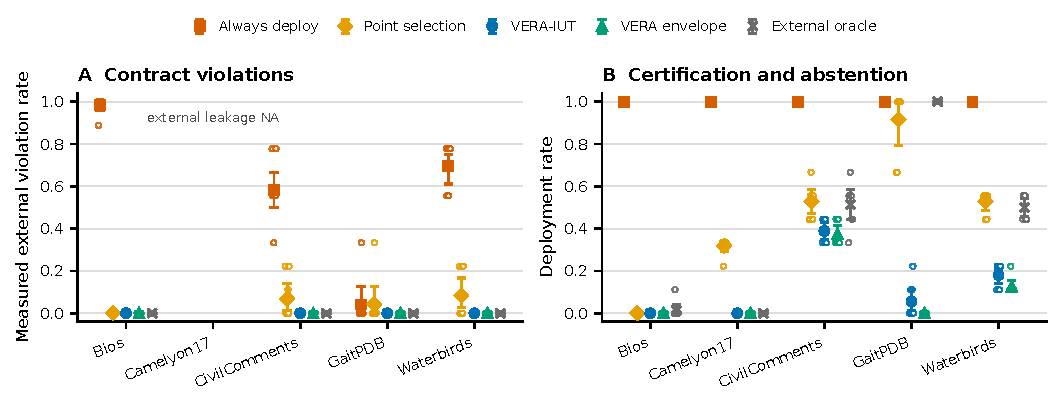
\includegraphics[width=\textwidth]{../../figures/vera_deployment_rules.pdf}
  \caption{\textbf{Deployment rules head to head.} Points are seed-cluster
  means and intervals resample seed clusters, preserving correlated thresholds
  and nested fractions within each cluster. Camelyon17 support mismatch is
  procedural non-certifiability, reported separately from measured external
  violations.}
  \label{fig:deployment-rules}
  \end{figure*}
}{
  \HeadlineResult

  The final paper reports the exact synthetic overlay first, followed by
  measured external contract violations and deployment retention for all
  decision rules. No proxy row or unreceipted estimate is eligible. Required
  ablations compare reduced and leave-one-out attacker portfolios, vary the
  shift budget and all nine locked threshold pairs,
  change certification size, summarize the groupwise certificate geometry,
  and remove each eraser family from the candidate frontier. These analyses
  do not tune on external outcomes.
}

\section{Reproducibility}

\CodeAvailabilityText Every claim-grade result is regenerated from a receipt
that records the locked parent commit, upstream eraser commit, split hashes,
and per-example audit-array hashes.

\paragraph{Generative-AI assistance disclosure.}
OpenAI Codex was used extensively for research ideation, literature discovery,
theorem and proof drafting, software implementation, experiment orchestration,
statistical-analysis code, figure and manuscript drafting, and editing. No AI
system is an author or a citable source. The human author or authors are
responsible for independently verifying every claim, proof, implementation,
reference, data right, and policy obligation before submission; that
verification remains an explicit pre-submission gate.

\section{Limitations and Conclusion}

VERA's guarantee is finite-sample but scoped. It assumes bounded audit
variables, a certification fold independent of edit and attacker construction,
and deployment support covered by certification. The density-ratio budget is a
declared sensitivity parameter, not an empirically discovered fact. A finite
attacker portfolio cannot prove that no measurable algorithm recovers the
concept, and suppressing registered leakage does not establish fairness for
unmeasured concepts. The Camelyon17 experiment is not clinical validation.
Finally, eight algorithmic seeds quantify fitting and split variation but do
not make the five benchmark datasets a random sample of deployment domains.
The primary sign-flip analysis relies on paired sign symmetry; a sign-only
sensitivity is also reported. Both were fixed before those seeds were run, and
all four adjusted values are reported regardless of outcome.

Within those boundaries, VERA changes the output of representation erasure
from ``apply this edit'' to a falsifiable statement: this edit meets these
paired target and attacker contracts up to this supported reweighting budget.
When the data cannot justify that sentence, abstention is the result rather
than a hidden limitation.
